\chapter{BIAS UNDER A MIXTURE MODEL AND ITS BEHAVIOR}\label{chap:bias_mixture}
%%%%%%%%%%%%%%%%%%%%%%%%%%%%%%%%%%%%%%%%%%%%%%%%%%%%%%%%%%%%%%%%%%%%%%%%%%%%%%%%%%%%%
%%%%%%%%%%%%%%%%%%%%%%%%%%%%%%%%%%%%%%%%%%%%%%%%%%%%%%%%%%%%%%%%%%%%%%%%%%%%%%%%%%%%%
%%%%%%%%%%%%%%%%%%%%%%%%%%%%%%%%%%%%%%%%%%%%%%%%%%%%%%%%%%%%%%%%%%%%%%%%%%%%%%%%%%%%%
%%%%%%%%%%%%%%%%%%%%%%%%%%%%%%%%%%%%%%%%%%%%%%%%%%%%%%%%%%%%%%%%%%%%%%%%%%%%%%%%%%%%%
%%%%%%%%%%%%%%%%%%%%%%%%%%%%%%%%%%%%%%%%%%%%%%%%%%%%%%%%%%%%%%%%%%%%%%%%%%%%%%%%%%%%%
\section{What Is a Mixture Model?}\label{sec:mixture_model}
\hspace{24pt} Mixture models can arise for multiple reasons. This could be due to bad sampling methods, diverse population, or it could be intended. In general, a mixture model represents a population with more than one distribution in it. For our purposes, we will be analyzing a bivariate mixture model that contains true, intended data, and contaminating, unwanted data. More formally, we can define a mixture model below.
\begin{definition}\label{def:mixture}
    Let $\vec{V}$ and $\vec{C}$ be bivariate random vectors from the valid distribution and contaminated distribution, respectively. Let $W\sim\text{Bernoulli}(p)$, where $p$ is the proportion of contamination. Then define a bivariate mixture model as $$\vec{M}=W\vec{C}+\left(1-W\right)\vec{V}.$$
\end{definition}
Consider the following scenario. Statisticians are collecting two statistics for undergraduate students at a university. They administer surveys randomly throughout campus without screening. There is a possibility that graduate students accidentally enter the sample unintended. Although the probability may be low, it still must be considered. This sample will contain a proportion ($p$) of unwanted, contaminated data. Assume that the distribution of each population is known where undergraduates are the valid data and the graduate students are the contaminating data, and $$\vec{V}\sim\text{Normal}\left(\vec{\mu} = \begin{bmatrix}0\\ 0\end{bmatrix},\;\Sigma = \begin{bmatrix}0.07 & -0.03\\ -0.03 & 0.05\end{bmatrix}\right)$$ $$\vec{C}\sim\text{Normal}\left(\vec{\mu} = \begin{bmatrix}2\\ 3 \end{bmatrix},\;\Sigma = \begin{bmatrix}0.03 & -0.05\\ -0.05 & 0.1\end{bmatrix}\right).$$ Taking a random sample from these populations and mixing accordingly, we can observe the results in Figure \ref{fig:mixPlots} below. In the first graph we are introducing no mixing, and is all the valid population. In the second graph there is half-valid, half-contaminated. The third graph contains all contaminated data, which would occur if the statistician samples the wrong population, entirely. This example of mixing illustrates the famous Simpson's Paradox. Notice the correlation is negative with no mixing, and as mixing is introduced the correlation becomes positive and then back to negative as the contamination takes over. This relationship between mixing and positive/negative correlation will be similar to the main results introduced throughout this chapter.
\begin{figure}[H]
    \centering
    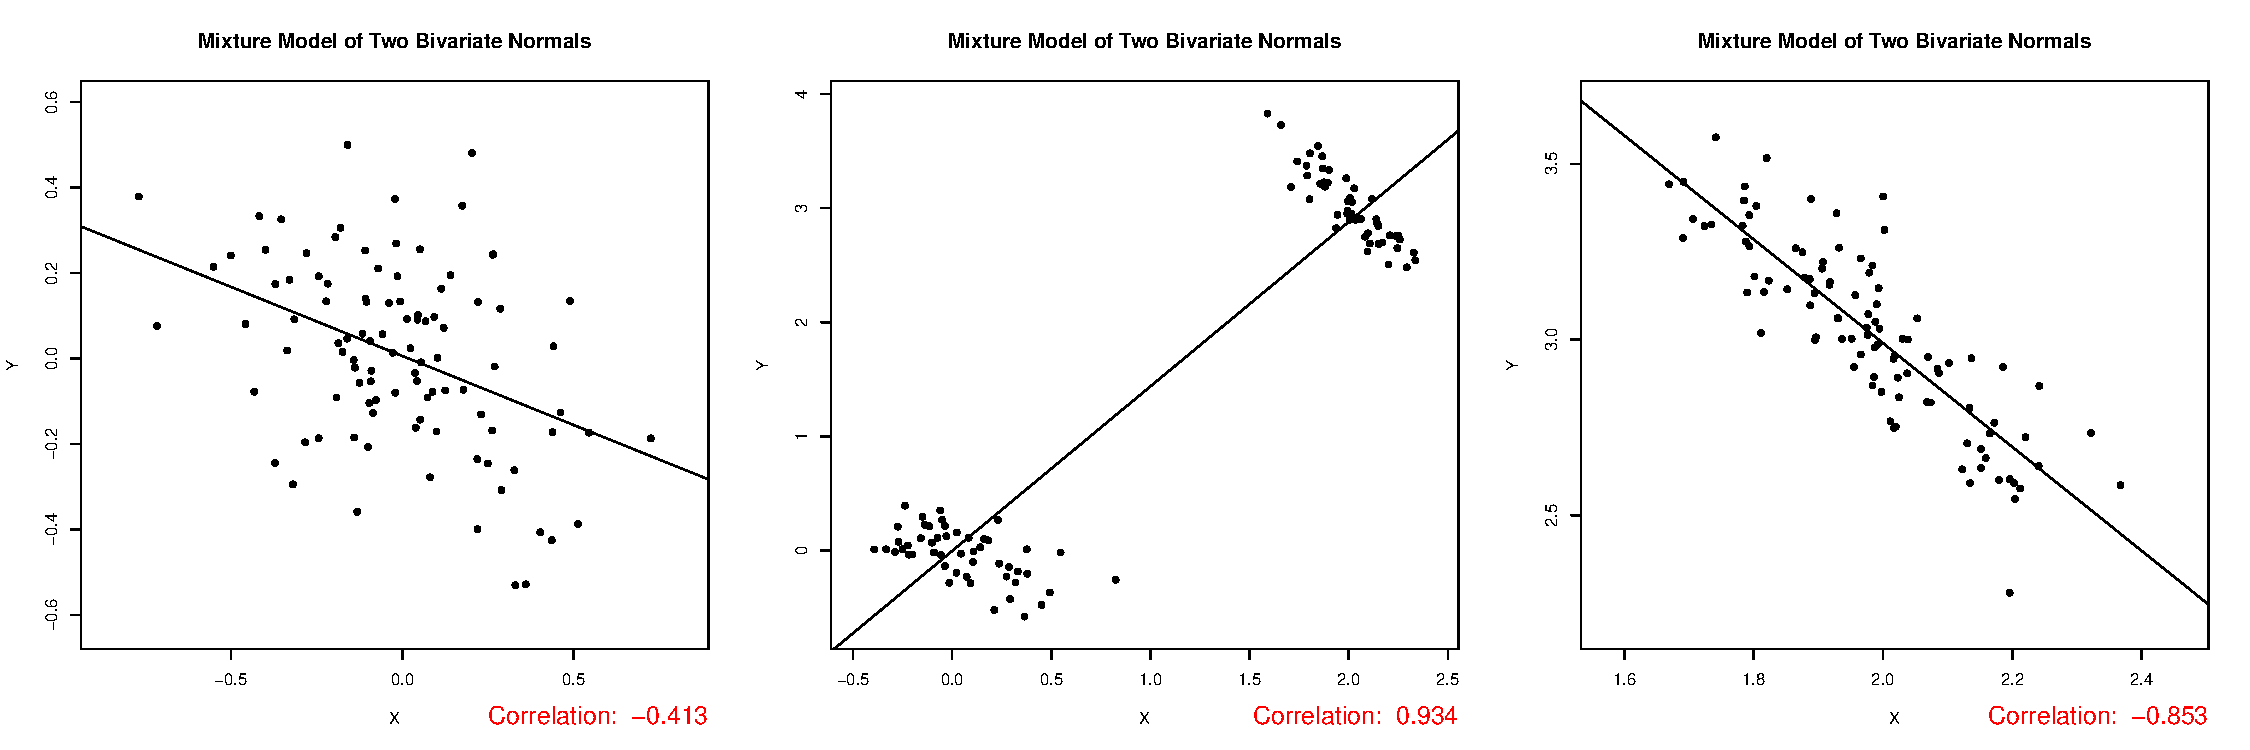
\includegraphics[scale=0.4]{images/mixturePlots.pdf}
    %\caption{Three different results of changing the mixing proportion ($p$). The first graph shows sampling the valid population. The second graph shows sampling half from the valid population and half from the contaminated population. The last graph shows sampling fully from the contaminated population. This diagram illustrates Simpson's Paradox. For visual convenience, the correlation is printed and the least-squares regression line is over-layed on each graph.}
    \caption{Three different results of changing the mixing proportion ($p$).}
    \label{fig:mixPlots}
\end{figure}
\hspace{24pt} The first graph shows sampling the valid population. The second graph shows sampling half from the valid population and half from the contaminated population. The last graph shows sampling fully from the contaminated population. This diagram illustrates Simpson's Paradox. For visual convenience, the correlation is printed and the least-squares regression line is over-layed on each graph.
%%%%%%%%%%%%%%%%%%%%%%%%%%%%%%%%%%%%%%%%%%%%%%%%%%%%%%%%%%%%%%%%%%%%%%%%%%%%%%%%%%%%%
%%%%%%%%%%%%%%%%%%%%%%%%%%%%%%%%%%%%%%%%%%%%%%%%%%%%%%%%%%%%%%%%%%%%%%%%%%%%%%%%%%%%%
%%%%%%%%%%%%%%%%%%%%%%%%%%%%%%%%%%%%%%%%%%%%%%%%%%%%%%%%%%%%%%%%%%%%%%%%%%%%%%%%%%%%%
%%%%%%%%%%%%%%%%%%%%%%%%%%%%%%%%%%%%%%%%%%%%%%%%%%%%%%%%%%%%%%%%%%%%%%%%%%%%%%%%%%%%%
%%%%%%%%%%%%%%%%%%%%%%%%%%%%%%%%%%%%%%%%%%%%%%%%%%%%%%%%%%%%%%%%%%%%%%%%%%%%%%%%%%%%%
\section{Bias Under Mixture Models}\label{sec:bias_mixtures}
\hspace{24pt} Traditionally, bias is defined as the difference between the expected value of an estimate and the true value of the parameter it is intended to estimate. In the context of Spearman's Rho, Kendall's Tau, and mixture models we define the bias as the difference between the parameter of the mixture and the parameter of the valid population. This can be defined more formally below.
\begin{definition}\label{def:bias_mixture}
    Let $\vec{V}$, $\vec{C}$, $\vec{M}$, $W$, and $p$ be described as in definition \ref{def:mixture}.  The bias under the mixture is
    \begin{align*}
        \text{Bias}_{\tau}(p)&=\tau_{\vec{M}}-\tau_{\vec{V}},\\
        \text{Bias}_{\rho}(p)&=\rho_{\vec{M}}-\rho_{\vec{V}}.
    \end{align*}
\end{definition}
Before the main result of the paper is introduced, there is one more lemma that will be used in the proof for Theorem \ref{theorem:main}. This lemma will use the property of the linearity of differentials and will help us prove later results.
\begin{lemma}\label{lem:differential}
    Let $f(x), g(x)$, and $h(x)$ be real-valued functions and let $a,b,c\in\mathbb{R}$. Then $$\int_s^t f(x)\mathrm{d}\left(ag(x)+bh(x)\right)=\int_s^t af(x)\mathrm{d}g(x)+\int_s^t bf(x)\mathrm{d}h(x).$$
\end{lemma}
Applying Definition \ref{def:bias_mixture} to the rank correlation methods, the main result of this paper can now be introduced.
\begin{theorem}\label{theorem:main}
    The bias in Kendall's Tau and Spearman's Rho due to mixing can be expressed as
    \begin{align*}
        \text{Bias}_{\tau}(p)&= 4\left(a_{\tau}p^2+b_{\tau}p\right)\\
        \text{Bias}_{\rho}(p)&= 12\left(a_{\rho}p^3+b_{\rho}p^2+c_{\rho}p\right),
    \end{align*}
    where
    \begin{align*}
        a_\tau=&\int\int_{\mathbb{R}^2}S_{\vec{V}}(x,y)\mathrm{d}S_{\vec{V}}(x,y)-\int\int_{\mathbb{R}^2}S_{\vec{V}}(x,y)\mathrm{d}S_{\vec{C}}(x,y)\\
        -&\int\int_{\mathbb{R}^2}S_{\vec{C}}(x,y)\mathrm{d}S_{\vec{V}}(x,y)+\int\int_{\mathbb{R}^2}S_{\vec{C}}(x,y)\mathrm{d}S_{\vec{C}}(x,y),\\
        b_\tau=&\int\int_{\mathbb{R}^2}S_{\vec{V}}(x,y)\mathrm{d}S_{\vec{C}}(x,y)+\int\int_{\mathbb{R}^2}S_{\vec{C}}(x,y)\mathrm{d}S_{\vec{V}}(x,y)\\
        -&2\int\int_{\mathbb{R}^2}S_{\vec{V}}(x,y)\mathrm{d}S_{\vec{V}}(x,y)
    \end{align*}
    and
    \begin{align*}
        a_\rho=&-\int\int_{\mathbb{R}^2}S_{\vec{V}}\left(x,y\right)\mathrm{d}S_{V_1}\left(x\right)\mathrm{d}S_{V_2}\left(y\right)+\int\int_{\mathbb{R}^2}S_{\vec{V}}\left(x,y\right)\mathrm{d}S_{V_1}\left(x\right)\mathrm{d}S_{C_2}\left(y\right)\\
        &+\int\int_{\mathbb{R}^2}S_{\vec{V}}\left(x,y\right)\mathrm{d}S_{C_1}\left(x\right)\mathrm{d}S_{V_2}\left(y\right)-\int\int_{\mathbb{R}^2}S_{\vec{V}}\left(x,y\right)\mathrm{d}S_{C_1}\left(x\right)\mathrm{d}S_{C_2}\left(y\right)\\
        &+\int\int_{\mathbb{R}^2}S_{\vec{C}}\left(x,y\right)\mathrm{d}S_{V_1}\left(x\right)\mathrm{d}S_{V_2}\left(y\right)-\int\int_{\mathbb{R}^2}S_{\vec{C}}\left(x,y\right)\mathrm{d}S_{V_1}\left(x\right)\mathrm{d}S_{C_2}\left(y\right)\\
        &-\int\int_{\mathbb{R}^2}S_{\vec{C}}\left(x,y\right)\mathrm{d}S_{C_1}\left(x\right)\mathrm{d}S_{V_2}\left(y\right)+\int\int_{\mathbb{R}^2}S_{\vec{C}}\left(x,y\right)\mathrm{d}S_{C_1}\left(x\right)\mathrm{d}S_{C_2}\left(y\right)\\
        b_\rho=&3\int\int_{\mathbb{R}^2}S_{\vec{V}}\left(x,y\right)\mathrm{d}S_{V_1}\left(x\right)\mathrm{d}S_{V_2}\left(y\right)-2\int\int_{\mathbb{R}^2}S_{\vec{V}}\left(x,y\right)\mathrm{d}S_{V_1}\left(x\right)\mathrm{d}S_{C_2}\left(y\right)\\
        &-2\int\int_{\mathbb{R}^2}S_{\vec{V}}\left(x,y\right)\mathrm{d}S_{C_1}\left(x\right)\mathrm{d}S_{V_2}\left(y\right)+\int\int_{\mathbb{R}^2}S_{\vec{V}}\left(x,y\right)\mathrm{d}S_{C_1}\left(x\right)\mathrm{d}S_{C_2}\left(y\right)\\
        &-2\int\int_{\mathbb{R}^2}S_{\vec{C}}\left(x,y\right)\mathrm{d}S_{V_1}\left(x\right)\mathrm{d}S_{V_2}\left(y\right)+\int\int_{\mathbb{R}^2}S_{\vec{C}}\left(x,y\right)\mathrm{d}S_{V_1}\left(x\right)\mathrm{d}S_{C_2}\left(y\right)\\
        &+\int\int_{\mathbb{R}^2}S_{\vec{C}}\left(x,y\right)\mathrm{d}S_{C_1}\left(x\right)\mathrm{d}S_{V_2}\left(y\right)\\
        c_\rho=&\int\int_{\mathbb{R}^2}S_{\vec{V}}\left(x,y\right)\mathrm{d}S_{V_1}\left(x\right)\mathrm{d}S_{C_2}\left(y\right)-3\int\int_{\mathbb{R}^2}S_{\vec{V}}\left(x,y\right)\mathrm{d}S_{V_1}\left(x\right)\mathrm{d}S_{V_2}\left(y\right)\\
        &+\int\int_{\mathbb{R}^2}S_{\vec{V}}\left(x,y\right)\mathrm{d}S_{C_1}\left(x\right)\mathrm{d}S_{V_2}\left(y\right)+\int\int_{\mathbb{R}^2}S_{\vec{C}}\left(x,y\right)\mathrm{d}S_{V_1}\left(x\right)\mathrm{d}S_{V_2}\left(y\right).
    \end{align*}
\end{theorem}
\begin{proof}
    Beginning with Kendall's Tau, we will start with the definition of bias.\\
    \begin{align*}
        \text{Bias}_{\tau}\left(p\right)=&\tau_{\vec{M}}-\tau_{\vec{V}}\\
        =&4\int\int_{\mathbb{R}^2}S_{\vec{M}}\left(x,y\right)\mathrm{d}S_{\vec{M}}\left(x,y\right)-1-\left(4\int\int_{\mathbb{R}^2}S_{\vec{V}}\left(x,y\right)\mathrm{d}S_{\vec{V}}\left(x,y\right)-1\right)\\
        =&4\int\int_{\mathbb{R}^2}\big[\left(1-p\right)S_{\vec{V}}\left(x,y\right)+pS_{\vec{C}}\left(x,y\right)\big]\mathrm{d}\left[\left(1-p\right)S_{\vec{V}}\left(x,y\right)+pS_{\vec{C}}\left(x,y\right)\right]\\
        &-4\int\int_{\mathbb{R}^2}S_{\vec{V}}\mathrm{d}S_{\vec{V}}\left(x,y\right).\\
    \end{align*}
    Now apply Lemma \ref{lem:differential}.
    \begin{align*}
        =&4\bigg[\int\int_{\mathbb{R}^2}\left(1-p\right)^2S_{\vec{V}}\left(x,y\right)\mathrm{d}S_{\vec{V}}\left(x,y\right)+\int\int_{\mathbb{R}^2}\left(1-p\right)pS_{\vec{V}}\left(x,y\right)\mathrm{d}S_{\vec{C}}\left(x,y\right)\\
        &+\int\int_{\mathbb{R}^2}p\left(1-p\right)S_{\vec{C}}\left(x,y\right)\mathrm{d}S_{\vec{V}}\left(x,y\right)+\int\int_{\mathbb{R}^2}p^2S_{\vec{C}}\left(x,y\right)\mathrm{d}S_{\vec{C}}\left(x,y\right)\bigg]\\
        &-4\int\int_{\mathbb{R}^2}S_{\vec{V}}\left(x,y\right)\mathrm{d}S_{\vec{V}}\left(x,y\right)\\
        =&4\bigg[\int\int_{\mathbb{R}^2}S_{\vec{V}}\left(x,y\right)\mathrm{d}S_{\vec{V}}\left(x,y\right)-2p\int\int_{\mathbb{R}^2}S_{\vec{V}}\left(x,y\right)\mathrm{d}S_{\vec{V}}\left(x,y\right)\\
        &+p^2\int\int_{\mathbb{R}^2}S_{\vec{V}}\left(x,y\right)\mathrm{d}S_{\vec{V}}\left(x,y\right)+p\int\int_{\mathbb{R}^2}S_{\vec{V}}\left(x,y\right)\mathrm{d}S_{\vec{C}}\left(x,y\right)\\
        &-p^2\int\int_{\mathbb{R}^2}S_{\vec{V}}\left(x,y\right)\mathrm{d}S_{\vec{C}}\left(x,y\right)+p\int\int_{\mathbb{R}^2}S_{\vec{C}}\left(x,y\right)\mathrm{d}S_{\vec{V}}\left(x,y\right)\\
        &-p^2\int\int_{\mathbb{R}^2}S_{\vec{C}}\left(x,y\right)\mathrm{d}S_{\vec{V}}\left(x,y\right)+p^2\int\int_{\mathbb{R}^2}S_{\vec{C}}\left(x,y\right)\mathrm{d}S_{\vec{C}}\left(x,y\right)\bigg]\\
        &-4\int\int_{\mathbb{R}^2}S_{\vec{V}}\left(x,y\right)\mathrm{d}S_{\vec{V}}\left(x,y\right)\\
        =&4\Bigg[p^2\bigg(\int\int_{\mathbb{R}^2}S_{\vec{V}}\left(x,y\right)\mathrm{d}S_{\vec{V}}\left(x,y\right)-\int\int_{\mathbb{R}^2}S_{\vec{V}}\left(x,y\right)\mathrm{d}S_{\vec{C}}\left(x,y\right)\\
        &-\int\int_{\mathbb{R}^2}S_{\vec{C}}\left(x,y\right)\mathrm{d}S_{\vec{V}}\left(x,y\right)+\int\int_{\mathbb{R}^2}S_{\vec{C}}\left(x,y\right)\mathrm{d}S_{\vec{C}}\left(x,y\right)\bigg)\\
        &+p\bigg(\int\int_{\mathbb{R}^2}S_{\vec{V}}\left(x,y\right)\mathrm{d}S_{\vec{C}}\left(x,y\right)+\int\int_{\mathbb{R}^2}S_{\vec{C}}\left(x,y\right)\mathrm{d}S_{\vec{V}}\left(x,y\right)\\
        &-2\int\int_{\mathbb{R}^2}S_{\vec{V}}\left(x,y\right)\mathrm{d}S_{\vec{V}}\left(x,y\right)\bigg)\Bigg]\\
        =&4\left(a_{\tau}p^2+b_{\tau}p\right).
    \end{align*}
    Using the same strategy above, we can use it solve for the bias of Rho under a mixture.
    \begin{align*}
        \text{Bias}_{\rho}\left(p\right)=&\rho_{\vec{M}}-\rho_{\vec{V}}\\
        =&12\int\int_{\mathbb{R}^2}S_{\vec{M}}\left(x,y\right)\mathrm{d}S_{M_1}\left(x\right)\mathrm{d}S_{M_2}\left(y\right)-3\\
        &-\left(12\int\int_{\mathbb{R}^2}S_{\vec{V}}\left(x,y\right)\mathrm{d}S_{V_1}\left(x\right)\mathrm{d}S_{V_2}\left(y\right)-3\right)\\
        =&12\int\int_{\mathbb{R}^2}\big[\left(1-p\right)S_{\vec{V}}\left(x,y\right)+pS_{\vec{C}}\left(x,y\right)\big]\\
        &\hspace{3cm}\mathrm{d}\big[\left(1-p\right)S_{V_1}\left(x\right)+pS_{C_1}\left(x\right)\big]\mathrm{d}\big[\left(1-p\right)S_{V_2}\left(y\right)+pS_{C_2}\left(y\right)\big]\\
        &-\left(12\int\int_{\mathbb{R}^2}S_{\vec{V}}\left(x,y\right)\mathrm{d}S_{V_1}\left(x\right)\mathrm{d}S_{V_2}\left(y\right)\right)\\
        =&12\bigg[\int\int_{\mathbb{R}^2}\left(1-p\right)^3S_{\vec{V}}\left(x,y\right)\mathrm{d}S_{V_1}\left(x\right)\mathrm{d}S_{V_2}\left(y\right)\\
        &+\int\int_{\mathbb{R}^2}\left(1-p\right)^2pS_{\vec{V}}\left(x,y\right)\mathrm{d}S_{V_1}\left(x\right)\mathrm{d}S_{C_2}\left(y\right)\\
        &+\int\int_{\mathbb{R}^2}\left(1-p\right)^2pS_{\vec{V}}\left(x,y\right)\mathrm{d}S_{C_1}\left(x\right)\mathrm{d}S_{V_2}\left(y\right)\\
        &+\int\int_{\mathbb{R}^2}\left(1-p\right)p^2S_{\vec{V}}\left(x,y\right)\mathrm{d}S_{C_1}\left(x\right)\mathrm{d}S_{C_2}\left(y\right)\\
        &+\int\int_{\mathbb{R}^2}\left(1-p\right)^2pS_{\vec{C}}\left(x,y\right)\mathrm{d}S_{V_1}\left(x\right)\mathrm{d}S_{V_2}\left(y\right)\\
        &+\int\int_{\mathbb{R}^2}p^2\left(1-p\right)S_{\vec{C}}\left(x,y\right)\mathrm{d}S_{V_1}\left(x\right)\mathrm{d}S_{C_2}\left(y\right)\\
        &+\int\int_{\mathbb{R}^2}p^2\left(1-p\right)S_{\vec{C}}\left(x,y\right)\mathrm{d}S_{C_1}\left(x\right)\mathrm{d}S_{V_2}\left(y\right)\\
        &+\int\int_{\mathbb{R}^2}p^3S_{\vec{C}}\left(x,y\right)\mathrm{d}S_{C_1}\left(x\right)\mathrm{d}S_{C_2}\left(y\right)\bigg]\\
        &-12\int\int_{\mathbb{R}^2}S_{\vec{V}}\left(x,y\right)\mathrm{d}S_{V_1}\left(x\right)\mathrm{d}S_{V_2}\left(y\right).
    \end{align*}
    \begin{align*}
        =&12\bigg[\int\int_{\mathbb{R}^2}S_{\vec{V}}\left(x,y\right)\mathrm{d}S_{V_1}\left(x\right)\mathrm{d}S_{V_2}\left(y\right)-3p\int\int_{\mathbb{R}^2}S_{\vec{V}}\left(x,y\right)\mathrm{d}S_{V_1}\left(x\right)\mathrm{d}S_{V_2}\left(y\right)\\
        &+3p^2\int\int_{\mathbb{R}^2}S_{\vec{V}}\left(x,y\right)\mathrm{d}S_{V_1}\left(x\right)\mathrm{d}S_{V_2}\left(y\right)-p^3\int\int_{\mathbb{R}^2}S_{\vec{V}}\left(x,y\right)\mathrm{d}S_{V_1}\left(x\right)\mathrm{d}S_{V_2}\left(y\right)\\
        &+p\int\int_{\mathbb{R}^2}S_{\vec{V}}\left(x,y\right)\mathrm{d}S_{V_1}\left(x\right)\mathrm{d}S_{C_2}\left(y\right)-2p^2\int\int_{\mathbb{R}^2}S_{\vec{V}}\left(x,y\right)\mathrm{d}S_{V_1}\left(x\right)\mathrm{d}S_{C_2}\left(y\right)\\
        &+p^3\int\int_{\mathbb{R}^2}S_{\vec{V}}\left(x,y\right)\mathrm{d}S_{V_1}\left(x\right)\mathrm{d}S_{C_2}\left(y\right)+p\int\int_{\mathbb{R}^2}S_{\vec{V}}\left(x,y\right)\mathrm{d}S_{C_1}\left(x\right)\mathrm{d}S_{V_2}\left(y\right)\\
        &-2p^2\int\int_{\mathbb{R}^2}S_{\vec{V}}\left(x,y\right)\mathrm{d}S_{C_1}\left(x\right)\mathrm{d}S_{V_2}\left(y\right)+p^3\int\int_{\mathbb{R}^2}S_{\vec{V}}\left(x,y\right)\mathrm{d}S_{C_1}\left(x\right)\mathrm{d}S_{V_2}\left(y\right)\\
        &+p^2\int\int_{\mathbb{R}^2}S_{\vec{V}}\left(x,y\right)\mathrm{d}S_{C_1}\left(x\right)\mathrm{d}S_{C_2}\left(y\right)-p^3\int\int_{\mathbb{R}^2}S_{\vec{V}}\left(x,y\right)\mathrm{d}S_{C_1}\left(x\right)\mathrm{d}S_{C_2}\left(y\right)\\
        &+p\int\int_{\mathbb{R}^2}S_{\vec{C}}\left(x,y\right)\mathrm{d}S_{V_1}\left(x\right)\mathrm{d}S_{V_2}\left(y\right)-2p^2\int\int_{\mathbb{R}^2}S_{\vec{C}}\left(x,y\right)\mathrm{d}S_{V_1}\left(x\right)\mathrm{d}S_{V_2}\left(y\right)\\
        &+p^3\int\int_{\mathbb{R}^2}S_{\vec{C}}\left(x,y\right)\mathrm{d}S_{V_1}\left(x\right)\mathrm{d}S_{V_2}\left(y\right)+p^2\int\int_{\mathbb{R}^2}S_{\vec{C}}\left(x,y\right)\mathrm{d}S_{V_1}\left(x\right)\mathrm{d}S_{C_2}\left(y\right)\\
        &-p^3\int\int_{\mathbb{R}^2}S_{\vec{C}}\left(x,y\right)\mathrm{d}S_{V_1}\left(x\right)\mathrm{d}S_{C_2}\left(y\right)+p^2\int\int_{\mathbb{R}^2}S_{\vec{C}}\left(x,y\right)\mathrm{d}S_{C_1}\left(x\right)\mathrm{d}S_{V_2}\left(Y\right)\\
        &-p^3\int\int_{\mathbb{R}^2}S_{\vec{C}}\left(x,y\right)\mathrm{d}S_{C_1}\left(x\right)\mathrm{d}S_{V_2}\left(y\right)+p^3\int\int_{\mathbb{R}^2}S_{\vec{C}}\left(x,y\right)\mathrm{d}S_{C_1}\left(x\right)\mathrm{d}S_{C_2}\left(y\right)\bigg]\\
        &-12\int\int_{\mathbb{R}^2}S_{\vec{V}}\left(x,y\right)\mathrm{d}S_{V_1}\left(x\right)\mathrm{d}S_{V_2}\left(y\right).
    \end{align*}
    \begin{align*}
        =&12\bigg[p^3\bigg(-\int\int_{\mathbb{R}^2}S_{\vec{V}}\left(x,y\right)\mathrm{d}S_{V_1}\left(x\right)\mathrm{d}S_{V_2}\left(y\right)+\int\int_{\mathbb{R}^2}S_{\vec{V}}\left(x,y\right)\mathrm{d}S_{V_1}\left(x\right)\mathrm{d}S_{C_2}\left(y\right)\\
        &+\int\int_{\mathbb{R}^2}S_{\vec{V}}\left(x,y\right)\mathrm{d}S_{C_1}\left(x\right)\mathrm{d}S_{V_2}\left(y\right)-\int\int_{\mathbb{R}^2}S_{\vec{V}}\left(x,y\right)\mathrm{d}S_{C_1}\left(x\right)\mathrm{d}S_{C_2}\left(y\right)\\
        &+\int\int_{\mathbb{R}^2}S_{\vec{C}}\left(x,y\right)\mathrm{d}S_{V_1}\left(x\right)\mathrm{d}S_{V_2}\left(y\right)-\int\int_{\mathbb{R}^2}S_{\vec{C}}\left(x,y\right)\mathrm{d}S_{V_1}\left(x\right)\mathrm{d}S_{C_2}\left(y\right)\\
        &-\int\int_{\mathbb{R}^2}S_{\vec{C}}\left(x,y\right)\mathrm{d}S_{C_1}\left(x\right)\mathrm{d}S_{V_2}\left(y\right)+\int\int_{\mathbb{R}^2}S_{\vec{C}}\left(x,y\right)\mathrm{d}S_{C_1}\left(x\right)\mathrm{d}S_{C_2}\left(y\right)\bigg)\\
        &+p^2\bigg(3\int\int_{\mathbb{R}^2}S_{\vec{V}}\left(x,y\right)\mathrm{d}S_{V_1}\left(x\right)\mathrm{d}S_{V_2}\left(y\right)-2\int\int_{\mathbb{R}^2}S_{\vec{V}}\left(x,y\right)\mathrm{d}S_{V_1}\left(x\right)\mathrm{d}S_{C_2}\left(y\right)\\
        &-2\int\int_{\mathbb{R}^2}S_{\vec{V}}\left(x,y\right)\mathrm{d}S_{C_1}\left(x\right)\mathrm{d}S_{V_2}\left(y\right)+\int\int_{\mathbb{R}^2}S_{\vec{V}}\left(x,y\right)\mathrm{d}S_{C_1}\left(x\right)\mathrm{d}S_{C_2}\left(y\right)\\
        &-2\int\int_{\mathbb{R}^2}S_{\vec{C}}\left(x,y\right)\mathrm{d}S_{V_1}\left(x\right)\mathrm{d}S_{V_2}\left(y\right)+\int\int_{\mathbb{R}^2}S_{\vec{C}}\left(x,y\right)\mathrm{d}S_{V_1}\left(x\right)\mathrm{d}S_{C_2}\left(y\right)\\
        &+\int\int_{\mathbb{R}^2}S_{\vec{C}}\left(x,y\right)\mathrm{d}S_{C_1}\left(x\right)\mathrm{d}S_{V_2}\left(y\right)\bigg)\\
        &+p\bigg(\int\int_{\mathbb{R}^2}S_{\vec{V}}\left(x,y\right)\mathrm{d}S_{V_1}\left(x\right)\mathrm{d}S_{C_2}\left(y\right)-3\int\int_{\mathbb{R}^2}S_{\vec{V}}\left(x,y\right)\mathrm{d}S_{V_1}\left(x\right)\mathrm{d}S_{V_2}\left(y\right)\\
        &+\int\int_{\mathbb{R}^2}S_{\vec{V}}\left(x,y\right)\mathrm{d}S_{C_1}\left(x\right)\mathrm{d}S_{V_2}\left(y\right)+\int\int_{\mathbb{R}^2}S_{\vec{C}}\left(x,y\right)\mathrm{d}S_{V_1}\left(x\right)\mathrm{d}S_{V_2}\left(y\right)\bigg)\bigg]\\
        =&12\left(a_{\rho}p^3+b_{\rho}p^2+c_{\rho}p\right).
    \end{align*}
\end{proof}
%%%%%%%%%%%%%%%%%%%%%%%%%%%%%%%%%%%%%%%%%%%%%%%%%%%%%%%%%%%%%%%%%%%%%%%%%%%%%%%%%%%%%
%%%%%%%%%%%%%%%%%%%%%%%%%%%%%%%%%%%%%%%%%%%%%%%%%%%%%%%%%%%%%%%%%%%%%%%%%%%%%%%%%%%%%
%%%%%%%%%%%%%%%%%%%%%%%%%%%%%%%%%%%%%%%%%%%%%%%%%%%%%%%%%%%%%%%%%%%%%%%%%%%%%%%%%%%%%
%%%%%%%%%%%%%%%%%%%%%%%%%%%%%%%%%%%%%%%%%%%%%%%%%%%%%%%%%%%%%%%%%%%%%%%%%%%%%%%%%%%%%
%%%%%%%%%%%%%%%%%%%%%%%%%%%%%%%%%%%%%%%%%%%%%%%%%%%%%%%%%%%%%%%%%%%%%%%%%%%%%%%%%%%%%
\section{General Behavior of Quadratics and Cubics}
\hspace{24pt} In the case of Tau, the final form expression for the bias is a quadratic without a constant term. In the case of Rho, the final form expression for the bias is a cubic without a constant term. For the interest of statistical application, it is common to want the sign of the bias. That is, whether the contamination will result in a positive or negative bias. By analyzing and characterizing all the different root behaviors, we can easily find the sign of the bias. Because the polynomials have no constant terms, our analysis will be simplified by having a root at zero.
\begin{prop}
    Consider a quadratic function without a constant term, $f(p)=ap^2+bp$. The following inequalities between $a$ and $b$ serve as a partition of the coefficient space that characterizes root behavior and thus the regions in the unit interval where the function is positive and negative. There are five cases below with subcases for some.
    \begin{enumerate}
        \item $f(p)=0$ for all $p$ in $(0,1)$. This occurs when $a=b=0$.
        \item $f(p)>0$ for all $p$ in $(0,1)$. This has two subcases.
        \begin{enumerate}
            \item $a\geq 0$ and $b\geq 0$ (but not both equal to zero).
            \item $0<-a\leq b$.
        \end{enumerate}
        \item $f(p)<0$ for all $p$ in $(0,1)$. This has two subcases.
        \begin{enumerate}
            \item $a\leq 0$ and $b\leq 0$ (but not both equal to zero).
            \item $b\leq -a<0$.
        \end{enumerate}
        \item There exists a root $p_1$ in $(0,1)$ such that $f(p)>0$ for $p<p_1$, but $f(p)<0$ for $p>p_1$.  This occurs when $0 < b < -a$. 
        \item There exists a non-zero root $p_1$ in $(0,1)$ such that $f(p) < 0$ for $p < p_1$, but $f(p) > 0$ for $p > p_1$.  This occurs when $-a < b < 0$.
    \end{enumerate}
    Consider a cubic function without a constant term, $f(p)=ap^3+bp^2 +cp$.  The following inequalities between $a,$ $b$, and $c$ serve as a partition of the coefficient space that characterizes root behavior and thus the regions in the unit interval where the function is positive and negative. There are 7 cases below with multiple subcases for some.
    \begin{enumerate}
        \item $f(p)=0$ for all $p$ in $(0,1)$. This occurs when $a=b=c=0$.
        \item $f(p)>0$ for all $p$ in $(0,1)$. This has four subcases.
        \begin{enumerate}
            \item $a>0$, $|b|<2\sqrt{ac}$, $c>0$.
            \item $a>0$, $|b|>2\sqrt{ac}$, $b\leq -2a$, $c\geq a$, $a+b+c\geq 0$.
            \item $a>0$, $b>0$, $c>0$, $|b|>2\sqrt{ac}$.
            \item $a<0$, $c>0$, $a+b+c\geq 0$.
        \end{enumerate}
        \item $f(p)<0$ for all $p$ in $(0,1)$. This has four subcases.
        \begin{enumerate}
            \item $a<0$, $|b|<2\sqrt{ac}$, $c<0$.
            \item $a<0$, $|b|>2\sqrt{ac}$, $b\geq -2a$, $c\leq a$, $a+b+c\leq 0$.
            \item $a<0$, $b<0$, $c<0$, $|b|>2\sqrt{ac}$.
            \item $a>0$, $c<0$, $a+b+c\leq 0$.
        \end{enumerate}
        \item There exists a non-zero root $p_1$ in $(0,1)$ such that $f(p)>0$ for $p<p_1$, but $f(p)<0$ for $p>p_1$. This has two subcases.
        \begin{enumerate}
            \item $a>0$, $b\leq -a$, $c>0$, $|b|>2\sqrt{ac}$, $a+b+c\leq0$.
            \item $a<0$, $c>0$, $a+b+c\leq 0$.
        \end{enumerate}
        \item There exists a non-zero root $p_1$ in $(0,1)$ such that $f(p)<0$ for $0<p<p_1$, but $f(p)>0$ for $p_1<p<1$. This has two subcases.
        \begin{enumerate}
            \item $a<0$, $b\geq -a$, $c<0$, $|b|>2\sqrt{ac}$, $a+b+c\geq 0$.
            \item $a>0$, $c<0$, $a+b+c\geq 0$.
        \end{enumerate}
        \item There exists two non-zero roots $p_1<p_2$ in $(0,1)$ such that $f(p)>0$ for $0<p<p_1$, $f(p)<0$ for $p_1<p<p_2$, and $f(p)>0$ for $p_2<p<1$. This occurs when $a>0$, $-2a\leq b\leq 0$, $c\leq a$, $|b|>2\sqrt{ac}$, $a+b+c\geq0$.
        \item There exists two non-zero roots $p_1<p_2$ in $(0,1)$ such that $f(p)<0$ for $0<p<p_1$, $f(p)>0$ for $p_1<p<p_2$, and $f(p)<0$ for $p_2<p<1$. This occurs when $a<0$, $-2a\geq b\geq 0$, $c\geq a$, $|b|>2\sqrt{ac}$, $a+b+c\leq 0$.
    \end{enumerate}
\end{prop}
The proof of these cases are elementary, yet tedious, and will be skipped. The application of these cases will be shown graphically in Chapter \ref{chap:MO} when we study the Marshall-Olkin distribution.